%%=============================================================================
%% LaTeX sjabloon voor bachelorproef, HoGent Bedrijf en Organisatie
%% Opleiding Toegepaste Informatica
%%=============================================================================

\documentclass[fleqn,a4paper,12pt]{book}

%%=============================================================================
%% LaTeX sjabloon voor de bachelorproef, HoGent Bedrijf en Organisatie
%% Opleiding toegepaste informatica
%%
%% Structuur en algemene vormgeving. Meestal hoef je hier niets te wijzigen.
%%
%% Vormgeving gebaseerd op "The Legrand Orange Book", version 2.0 (9/2/15)
%% door Mathias Legrand (legrand.mathias@gmail.com) met aanpassingen door
%% Vel (vel@latextemplates.com). Het oorspronkelijke template is te vinden op
%% http://www.LaTeXTemplates.com
%%
%% Aanpassingen voor HoGent toegepaste informatica: 
%%   Bert Van Vreckem <bert.vanvreckem@hogent.be>
%% Licentie: 
%%   CC BY-NC-SA 3.0 (http://creativecommons.org/licenses/by-nc-sa/3.0/)
%%=============================================================================

%%-----------------------------------------------------------------------------
%% Packages
%%-----------------------------------------------------------------------------

\usepackage[top=3cm,bottom=3cm,left=3cm,right=3cm,headsep=10pt,a4paper]{geometry} % Page margins
\usepackage[utf8]{inputenc}  % Accenten gebruiken in tekst (vb. é ipv \'e)
\usepackage{amsfonts}        % AMS math packages: extra wiskundige
\usepackage{amsmath}         %   symbolen (o.a. getallen-
\usepackage{amssymb}         %   verzamelingen N, R, Z, Q, etc.)
\usepackage[english,dutch]{babel}    % Taalinstellingen: woordsplitsingen,
                             %  commando's voor speciale karakters
                             %  ("dutch" voor NL)
\usepackage{iflang}
\usepackage{eurosym}         % Euro-symbool €
\usepackage{geometry}
\usepackage{graphicx}        % Invoegen van tekeningen
\graphicspath{{img/}}       % Specifies the directory where pictures are stored
\usepackage{tikz}            % Required for drawing custom shapes
\usepackage[pdftex,bookmarks=true]{hyperref}
                             % PDF krijgt klikbare links & verwijzingen,
                             %  inhoudstafel
\usepackage{enumitem}        % Customize lists
\setlist{nolistsep}         % Reduce spacing between list items
\usepackage{listings}        % Broncode mooi opmaken
\usepackage{multirow}        % Tekst over verschillende cellen in tabellen
\usepackage{rotating}        % Tabellen en figuren roteren

\usepackage{booktabs}        % Required for nicer horizontal rules in tables

\usepackage{xcolor}          % Required for specifying colors by name
\definecolor{maincolor}{RGB}{0,147,208} % Define the main color used for 
                             % highlighting throughout the book
                             % 0, 147, 208 = officiële kleur HoGent FBO

% Paragraph style: no indent, add space between paragraphs
\setlength{\parindent}{0em}
\setlength{\parskip}{1em}

\usepackage{etoolbox}
\usepackage{titling} % Macros for title, author, etc
\usepackage{lipsum}          % Voor vultekst (lorem ipsum)

%----------------------------------------------------------------------------------------
%	FONTS
%----------------------------------------------------------------------------------------

\usepackage{avant} % Use the Avantgarde font for headings
%\usepackage{times} % Use the Times font for headings
\usepackage{mathptmx} % Use the Adobe Times Roman as the default text font together with math symbols from the Sym­bol, Chancery and Com­puter Modern fonts

\usepackage{microtype} % Slightly tweak font spacing for aesthetics
\usepackage[utf8]{inputenc} % Required for including letters with accents
\usepackage[T1]{fontenc} % Use 8-bit encoding that has 256 glyphs

%----------------------------------------------------------------------------------------
%	CUSTOM PACKAGES
%----------------------------------------------------------------------------------------
\usepackage{listings}
\usepackage{caption}
\usepackage{subcaption}
\usepackage{pythonhighlight}
\usepackage[acronym]{glossaries}

%------------------------------------------------------------------------------
%	TITLE PAGE
%------------------------------------------------------------------------------

\newcommand{\inserttitlepage}{%
\begin{titlepage}
  \newgeometry{top=2cm,bottom=1.5cm,left=1.5cm,right=1.5cm}
  \begin{center}

    \begingroup
    \rmfamily
    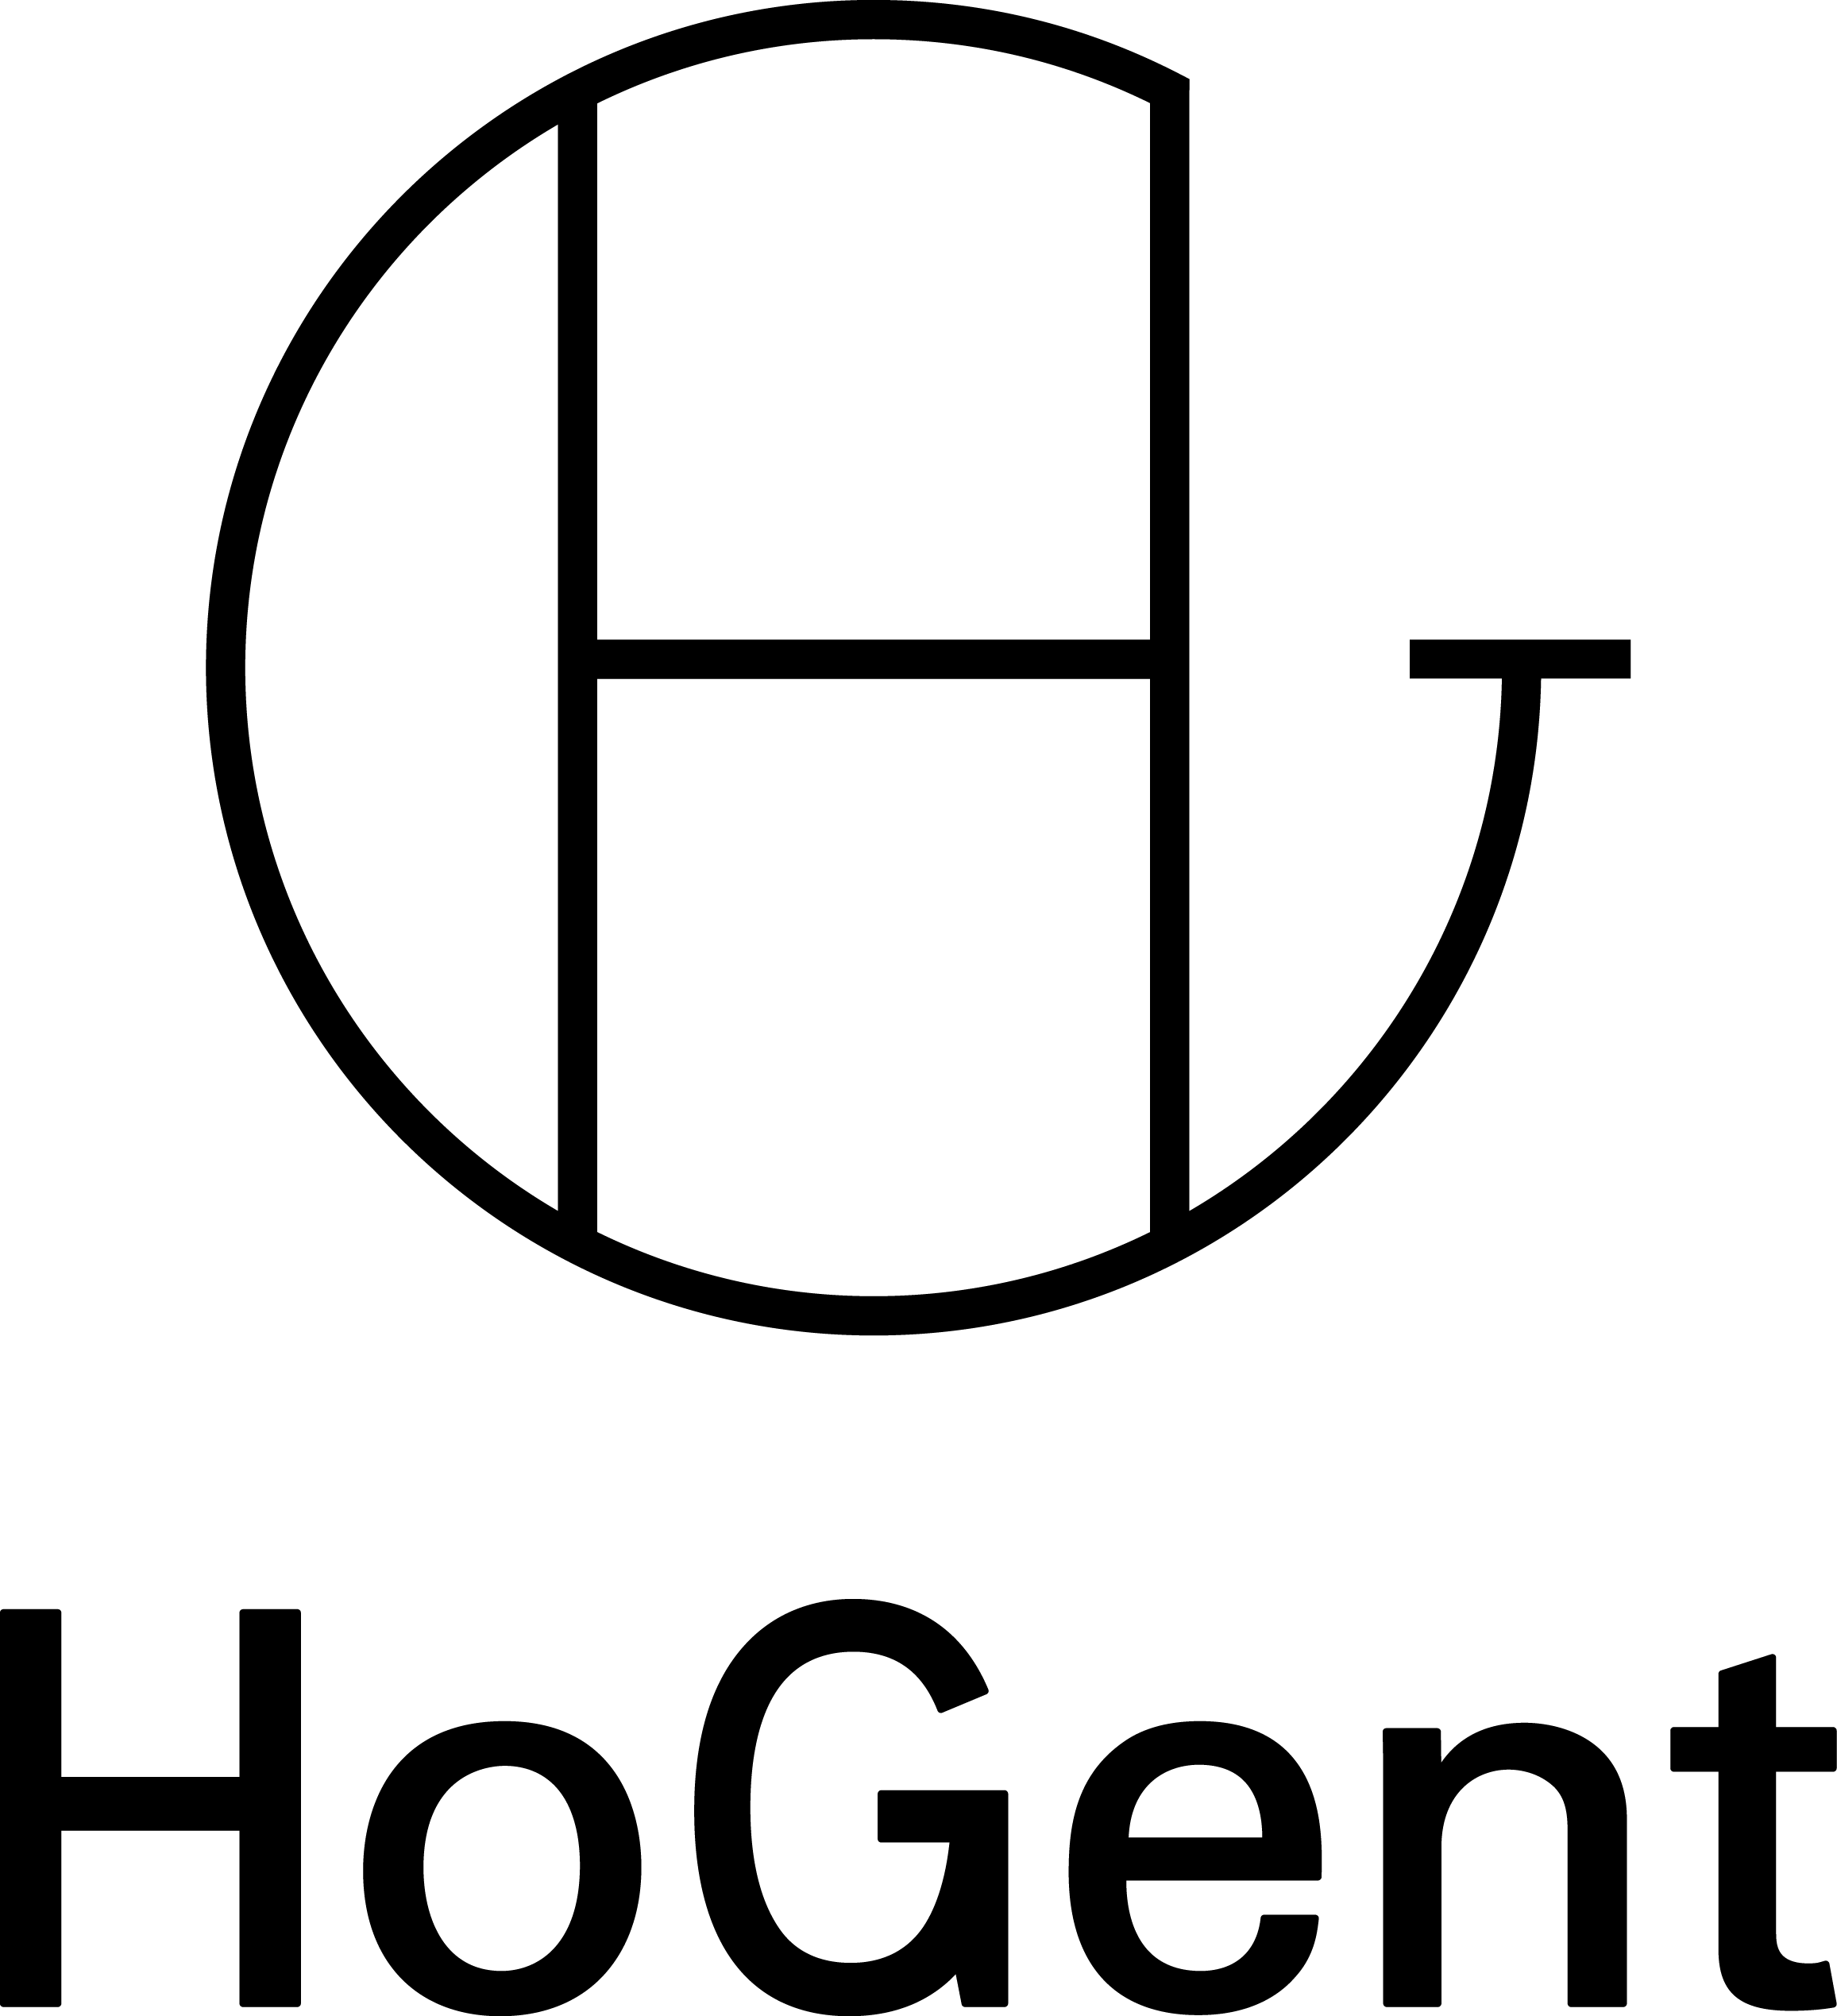
\includegraphics[width=2.5cm]{img/HG-beeldmerk-woordmerk}\\[.5cm]
    Faculteit Bedrijf en Organisatie\\[3cm]
    \titel
    \vfill
    \student\\[3.5cm]
    Scriptie voorgedragen tot het bekomen van de graad van\\professionele bachelor in de toegepaste informatica\\[2cm]
    Promotor:\\
    \promotor\\
    \ifdefempty{\copromotor}{\vspace{2.5cm}}{Co-promotor:\\\copromotor\\[2.5cm]}
    Instelling: \instelling\\[.5cm]
    Academiejaar: \academiejaar\\[.5cm]
    \ifcase \examenperiode \or Eerste \or Tweede \else Derde \fi examenperiode
    \endgroup

  \end{center}
  \restoregeometry
\end{titlepage}
  \emptypage
\begin{titlepage}
  \newgeometry{top=5.35cm,bottom=1.5cm,left=1.5cm,right=1.5cm}
  \begin{center}

    \begingroup
    \rmfamily
    \IfLanguageName{dutch}{Faculteit Bedrijf en Organisatie}{Faculty of Business and Information Management}\\[3cm]
    \titel
    \vfill
    \student\\[3.5cm]
    \IfLanguageName{dutch}{Scriptie voorgedragen tot het bekomen van de graad van\\professionele bachelor in de toegepaste informatica}{Thesis submitted in partial fulfilment of the requirements for the degree of\\professional bachelor of applied computer science}\\[2cm]
    Promotor:\\
    \promotor\\
    \ifdefempty{\copromotor}{\vspace{2.5cm}}{Co-promotor:\\\copromotor\\[2.5cm]}
    \IfLanguageName{dutch}{Instelling}{Institution}: \instelling\\[.5cm]
    \IfLanguageName{dutch}{Academiejaar}{Academic year}: \academiejaar\\[.5cm]
    \IfLanguageName{dutch}{%
    \ifcase \examenperiode \or Eerste \or Tweede \else Derde \fi examenperiode}{%
    \ifcase \examenperiode \or First \or Second \else Third \fi examination period}
    \endgroup

  \end{center}
  \restoregeometry
\end{titlepage}
}

%----------------------------------------------------------------------------------------
%	BIBLIOGRAPHY AND INDEX
%----------------------------------------------------------------------------------------

\usepackage[style=apa,backend=biber]{biblatex}
\usepackage{csquotes}
\DeclareLanguageMapping{dutch}{dutch-apa}
\addbibresource{bachproef-tin.bib} % BibTeX bibliography file
\addbibresource{../voorstel/voorstel.bib}
\defbibheading{bibempty}{}

\usepackage{calc} % For simpler calculation - used for spacing the index letter headings correctly
\usepackage{makeidx} % Required to make an index
\makeindex % Tells LaTeX to create the files required for indexing

%----------------------------------------------------------------------------------------
%	MAIN TABLE OF CONTENTS
%----------------------------------------------------------------------------------------

\usepackage{titletoc} % Required for manipulating the table of contents

\contentsmargin{0cm} % Removes the default margin

% Part text styling
\titlecontents{part}[0cm]
{\addvspace{20pt}\centering\large\bfseries}
{}
{}
{}

% Chapter text styling
\titlecontents{chapter}[1.25cm] % Indentation
{\addvspace{12pt}\large\sffamily\bfseries} % Spacing and font options for chapters
{\color{maincolor!60}\contentslabel[\Large\thecontentslabel]{1.25cm}\color{maincolor}} % Chapter number
{\color{maincolor}}
{\color{maincolor!60}\normalsize\;\titlerule*[.5pc]{.}\;\thecontentspage} % Page number

% Section text styling
\titlecontents{section}[1.25cm] % Indentation
{\addvspace{3pt}\sffamily\bfseries} % Spacing and font options for sections
{\contentslabel[\thecontentslabel]{1.25cm}} % Section number
{}
{\hfill\color{black}\thecontentspage} % Page number
[]

% Subsection text styling
\titlecontents{subsection}[1.25cm] % Indentation
{\addvspace{1pt}\sffamily\small} % Spacing and font options for subsections
{\contentslabel[\thecontentslabel]{1.25cm}} % Subsection number
{}
{\ \titlerule*[.5pc]{.}\;\thecontentspage} % Page number
[]

% List of figures
\titlecontents{figure}[0em]
{\addvspace{-5pt}\sffamily}
{\thecontentslabel\hspace*{1em}}
{}
{\ \titlerule*[.5pc]{.}\;\thecontentspage}
[]

% List of tables
\titlecontents{table}[0em]
{\addvspace{-5pt}\sffamily}
{\thecontentslabel\hspace*{1em}}
{}
{\ \titlerule*[.5pc]{.}\;\thecontentspage}
[]

%----------------------------------------------------------------------------------------
%	MINI TABLE OF CONTENTS IN PART HEADS
%----------------------------------------------------------------------------------------

% Chapter text styling
\titlecontents{lchapter}[0em] % Indenting
{\addvspace{15pt}\large\sffamily\bfseries} % Spacing and font options for chapters
{\color{maincolor}\contentslabel[\Large\thecontentslabel]{1.25cm}\color{maincolor}} % Chapter number
{}
{\color{maincolor}\normalsize\sffamily\bfseries\;\titlerule*[.5pc]{.}\;\thecontentspage} % Page number

% Section text styling
\titlecontents{lsection}[0em] % Indenting
{\sffamily\small} % Spacing and font options for sections
{\contentslabel[\thecontentslabel]{1.25cm}} % Section number
{}
{}

% Subsection text styling
\titlecontents{lsubsection}[.5em] % Indentation
{\normalfont\footnotesize\sffamily} % Font settings
{}
{}
{}

%----------------------------------------------------------------------------------------
%	PAGE HEADERS
%----------------------------------------------------------------------------------------

\usepackage{fancyhdr} % Required for header and footer configuration

\pagestyle{fancy}
\renewcommand{\chaptermark}[1]{\markboth{\sffamily\normalsize\bfseries\chaptername\ \thechapter.\ #1}{}} % Chapter text font settings
\renewcommand{\sectionmark}[1]{\markright{\sffamily\normalsize\thesection\hspace{5pt}#1}{}} % Section text font settings
\fancyhf{} \fancyhead[LE,RO]{\sffamily\normalsize\thepage} % Font setting for the page number in the header
\fancyhead[LO]{\rightmark} % Print the nearest section name on the left side of odd pages
\fancyhead[RE]{\leftmark} % Print the current chapter name on the right side of even pages
\renewcommand{\headrulewidth}{0.5pt} % Width of the rule under the header
\addtolength{\headheight}{2.5pt} % Increase the spacing around the header slightly
\renewcommand{\footrulewidth}{0pt} % Removes the rule in the footer
\fancypagestyle{plain}{\fancyhead{}\renewcommand{\headrulewidth}{0pt}} % Style for when a plain pagestyle is specified

% Removes the header from odd empty pages at the end of chapters
\makeatletter
\renewcommand{\cleardoublepage}{
\clearpage\ifodd\c@page\else
\hbox{}
\vspace*{\fill}
\thispagestyle{empty}
\newpage
\fi}

%----------------------------------------------------------------------------------------
%	THEOREM STYLES
%----------------------------------------------------------------------------------------

\usepackage{amsmath,amsfonts,amssymb,amsthm} % For math equations, theorems, symbols, etc

\newcommand{\intoo}[2]{\mathopen{]}#1\,;#2\mathclose{[}}
\newcommand{\ud}{\mathop{\mathrm{{}d}}\mathopen{}}
\newcommand{\intff}[2]{\mathopen{[}#1\,;#2\mathclose{]}}
\newtheorem{notation}{Notation}[chapter]

% Boxed/framed environments
\newtheoremstyle{maincolornumbox}% % Theorem style name
{0pt}% Space above
{0pt}% Space below
{\normalfont}% % Body font
{}% Indent amount
{\small\bf\sffamily\color{maincolor}}% % Theorem head font
{\;}% Punctuation after theorem head
{0.25em}% Space after theorem head
{\small\sffamily\color{maincolor}\thmname{#1}\nobreakspace\thmnumber{\@ifnotempty{#1}{}\@upn{#2}}% Theorem text (e.g. Theorem 2.1)
\thmnote{\nobreakspace\the\thm@notefont\sffamily\bfseries\color{black}---\nobreakspace#3.}} % Optional theorem note
\renewcommand{\qedsymbol}{$\blacksquare$}% Optional qed square

\newtheoremstyle{blacknumex}% Theorem style name
{5pt}% Space above
{5pt}% Space below
{\normalfont}% Body font
{} % Indent amount
{\small\bf\sffamily}% Theorem head font
{\;}% Punctuation after theorem head
{0.25em}% Space after theorem head
{\small\sffamily{\tiny\ensuremath{\blacksquare}}\nobreakspace\thmname{#1}\nobreakspace\thmnumber{\@ifnotempty{#1}{}\@upn{#2}}% Theorem text (e.g. Theorem 2.1)
\thmnote{\nobreakspace\the\thm@notefont\sffamily\bfseries---\nobreakspace#3.}}% Optional theorem note

\newtheoremstyle{blacknumbox} % Theorem style name
{0pt}% Space above
{0pt}% Space below
{\normalfont}% Body font
{}% Indent amount
{\small\bf\sffamily}% Theorem head font
{\;}% Punctuation after theorem head
{0.25em}% Space after theorem head
{\small\sffamily\thmname{#1}\nobreakspace\thmnumber{\@ifnotempty{#1}{}\@upn{#2}}% Theorem text (e.g. Theorem 2.1)
\thmnote{\nobreakspace\the\thm@notefont\sffamily\bfseries---\nobreakspace#3.}}% Optional theorem note

% Non-boxed/non-framed environments
\newtheoremstyle{maincolornum}% % Theorem style name
{5pt}% Space above
{5pt}% Space below
{\normalfont}% % Body font
{}% Indent amount
{\small\bf\sffamily\color{maincolor}}% % Theorem head font
{\;}% Punctuation after theorem head
{0.25em}% Space after theorem head
{\small\sffamily\color{maincolor}\thmname{#1}\nobreakspace\thmnumber{\@ifnotempty{#1}{}\@upn{#2}}% Theorem text (e.g. Theorem 2.1)
\thmnote{\nobreakspace\the\thm@notefont\sffamily\bfseries\color{black}---\nobreakspace#3.}} % Optional theorem note
\renewcommand{\qedsymbol}{$\blacksquare$}% Optional qed square
\makeatother

% Defines the theorem text style for each type of theorem to one of the three styles above
\newcounter{dummy}
\numberwithin{dummy}{section}
\theoremstyle{maincolornumbox}
\newtheorem{theoremeT}[dummy]{Theorem}
\newtheorem{problem}{Problem}[chapter]
\newtheorem{exerciseT}{Exercise}[chapter]
\theoremstyle{blacknumex}
\newtheorem{exampleT}{Example}[chapter]
\theoremstyle{blacknumbox}
\newtheorem{vocabulary}{Vocabulary}[chapter]
\newtheorem{definitionT}{Definition}[section]
\newtheorem{corollaryT}[dummy]{Corollary}
\theoremstyle{maincolornum}
\newtheorem{proposition}[dummy]{Proposition}

%----------------------------------------------------------------------------------------
%	DEFINITION OF COLORED BOXES
%----------------------------------------------------------------------------------------

\RequirePackage[framemethod=default]{mdframed} % Required for creating the theorem, definition, exercise and corollary boxes

% Theorem box
\newmdenv[skipabove=7pt,
skipbelow=7pt,
backgroundcolor=black!5,
linecolor=maincolor,
innerleftmargin=5pt,
innerrightmargin=5pt,
innertopmargin=5pt,
leftmargin=0cm,
rightmargin=0cm,
innerbottommargin=5pt]{tBox}

% Exercise box
\newmdenv[skipabove=7pt,
skipbelow=7pt,
rightline=false,
leftline=true,
topline=false,
bottomline=false,
backgroundcolor=maincolor!10,
linecolor=maincolor,
innerleftmargin=5pt,
innerrightmargin=5pt,
innertopmargin=5pt,
innerbottommargin=5pt,
leftmargin=0cm,
rightmargin=0cm,
linewidth=4pt]{eBox}

% Definition box
\newmdenv[skipabove=7pt,
skipbelow=7pt,
rightline=false,
leftline=true,
topline=false,
bottomline=false,
linecolor=maincolor,
innerleftmargin=5pt,
innerrightmargin=5pt,
innertopmargin=0pt,
leftmargin=0cm,
rightmargin=0cm,
linewidth=4pt,
innerbottommargin=0pt]{dBox}

% Corollary box
\newmdenv[skipabove=7pt,
skipbelow=7pt,
rightline=false,
leftline=true,
topline=false,
bottomline=false,
linecolor=gray,
backgroundcolor=black!5,
innerleftmargin=5pt,
innerrightmargin=5pt,
innertopmargin=5pt,
leftmargin=0cm,
rightmargin=0cm,
linewidth=4pt,
innerbottommargin=5pt]{cBox}

% Creates an environment for each type of theorem and assigns it a theorem text style from the "Theorem Styles" section above and a colored box from above
\newenvironment{theorem}{\begin{tBox}\begin{theoremeT}}{\end{theoremeT}\end{tBox}}
\newenvironment{exercise}{\begin{eBox}\begin{exerciseT}}{\hfill{\color{maincolor}\tiny\ensuremath{\blacksquare}}\end{exerciseT}\end{eBox}}
\newenvironment{definition}{\begin{dBox}\begin{definitionT}}{\end{definitionT}\end{dBox}}
\newenvironment{example}{\begin{exampleT}}{\hfill{\tiny\ensuremath{\blacksquare}}\end{exampleT}}
\newenvironment{corollary}{\begin{cBox}\begin{corollaryT}}{\end{corollaryT}\end{cBox}}

%----------------------------------------------------------------------------------------
%	REMARK ENVIRONMENT
%----------------------------------------------------------------------------------------

\newenvironment{remark}{\par\vspace{10pt}\small % Vertical white space above the remark and smaller font size
\begin{list}{}{
\leftmargin=35pt % Indentation on the left
\rightmargin=25pt}\item\ignorespaces % Indentation on the right
\makebox[-2.5pt]{\begin{tikzpicture}[overlay]
\node[draw=maincolor!60,line width=1pt,circle,fill=maincolor!25,font=\sffamily\bfseries,inner sep=2pt,outer sep=0pt] at (-15pt,0pt){\textcolor{maincolor}{R}};\end{tikzpicture}} % Orange R in a circle
\advance\baselineskip -1pt}{\end{list}\vskip5pt} % Tighter line spacing and white space after remark

%----------------------------------------------------------------------------------------
%	SECTION NUMBERING IN THE MARGIN
%----------------------------------------------------------------------------------------

\makeatletter
\renewcommand{\@seccntformat}[1]{\llap{\textcolor{maincolor}{\csname the#1\endcsname}\hspace{1em}}}
\renewcommand{\section}{\@startsection{section}{1}{\z@}
{-4ex \@plus -1ex \@minus -.4ex}
{1ex \@plus.2ex }
{\normalfont\large\sffamily\bfseries}}
\renewcommand{\subsection}{\@startsection {subsection}{2}{\z@}
{-3ex \@plus -0.1ex \@minus -.4ex}
{0.5ex \@plus.2ex }
{\normalfont\sffamily\bfseries}}
\renewcommand{\subsubsection}{\@startsection {subsubsection}{3}{\z@}
{-2ex \@plus -0.1ex \@minus -.2ex}
{.2ex \@plus.2ex }
{\normalfont\small\sffamily\bfseries}}
\renewcommand\paragraph{\@startsection{paragraph}{4}{\z@}
{-2ex \@plus-.2ex \@minus .2ex}
{.1ex}
{\normalfont\small\sffamily\bfseries}}

%----------------------------------------------------------------------------------------
%	PART HEADINGS
%----------------------------------------------------------------------------------------

% numbered part in the table of contents
\newcommand{\@mypartnumtocformat}[2]{%
\setlength\fboxsep{0pt}%
\noindent\colorbox{maincolor!20}{\strut\parbox[c][.7cm]{\ecart}{\color{maincolor!70}\Large\sffamily\bfseries\centering#1}}\hskip\esp\colorbox{maincolor!40}{\strut\parbox[c][.7cm]{\linewidth-\ecart-\esp}{\Large\sffamily\centering#2}}}%
%%%%%%%%%%%%%%%%%%%%%%%%%%%%%%%%%%
% unnumbered part in the table of contents
\newcommand{\@myparttocformat}[1]{%
\setlength\fboxsep{0pt}%
\noindent\colorbox{maincolor!40}{\strut\parbox[c][.7cm]{\linewidth}{\Large\sffamily\centering#1}}}%
%%%%%%%%%%%%%%%%%%%%%%%%%%%%%%%%%%
\newlength\esp
\setlength\esp{4pt}
\newlength\ecart
\setlength\ecart{1.2cm-\esp}
\newcommand{\thepartimage}{}%
\newcommand{\partimage}[1]{\renewcommand{\thepartimage}{#1}}%
\def\@part[#1]#2{%
\ifnum \c@secnumdepth >-2\relax%
\refstepcounter{part}%
\addcontentsline{toc}{part}{\texorpdfstring{\protect\@mypartnumtocformat{\thepart}{#1}}{\partname~\thepart\ ---\ #1}}
\else%
\addcontentsline{toc}{part}{\texorpdfstring{\protect\@myparttocformat{#1}}{#1}}%
\fi%
\startcontents%
\markboth{}{}%
{\thispagestyle{empty}%
\begin{tikzpicture}[remember picture,overlay]%
\node at (current page.north west){\begin{tikzpicture}[remember picture,overlay]%
\fill[maincolor!20](0cm,0cm) rectangle (\paperwidth,-\paperheight);
\node[anchor=north] at (4cm,-3.25cm){\color{maincolor!40}\fontsize{220}{100}\sffamily\bfseries\@Roman\c@part};
\node[anchor=south east] at (\paperwidth-1cm,-\paperheight+1cm){\parbox[t][][t]{8.5cm}{
\printcontents{l}{0}{\setcounter{tocdepth}{1}}%
}};
\node[anchor=north east] at (\paperwidth-1.5cm,-3.25cm){\parbox[t][][t]{15cm}{\strut\raggedleft\color{white}\fontsize{30}{30}\sffamily\bfseries#2}};
\end{tikzpicture}};
\end{tikzpicture}}%
\@endpart}
\def\@spart#1{%
\startcontents%
\phantomsection
{\thispagestyle{empty}%
\begin{tikzpicture}[remember picture,overlay]%
\node at (current page.north west){\begin{tikzpicture}[remember picture,overlay]%
\fill[maincolor!20](0cm,0cm) rectangle (\paperwidth,-\paperheight);
\node[anchor=north east] at (\paperwidth-1.5cm,-3.25cm){\parbox[t][][t]{15cm}{\strut\raggedleft\color{white}\fontsize{30}{30}\sffamily\bfseries#1}};
\end{tikzpicture}};
\end{tikzpicture}}
\addcontentsline{toc}{part}{\texorpdfstring{%
\setlength\fboxsep{0pt}%
\noindent\protect\colorbox{maincolor!40}{\strut\protect\parbox[c][.7cm]{\linewidth}{\Large\sffamily\protect\centering #1\quad\mbox{}}}}{#1}}%
\@endpart}
\def\@endpart{\vfil\newpage
\if@twoside
\if@openright
\null
\thispagestyle{empty}%
\newpage
\fi
\fi
\if@tempswa
\twocolumn
\fi}

%----------------------------------------------------------------------------------------
%	CHAPTER HEADINGS
%----------------------------------------------------------------------------------------

% A switch to conditionally include a picture, implemented by  Christian Hupfer
\newif\ifusechapterimage
\usechapterimagetrue
\newcommand{\thechapterimage}{}%
\newcommand{\chapterimage}[1]{\ifusechapterimage\renewcommand{\thechapterimage}{#1}\fi}%
\def\@makechapterhead#1{%
{\parindent \z@ \raggedright \normalfont
\ifnum \c@secnumdepth >\m@ne
\if@mainmatter
\begin{tikzpicture}[remember picture,overlay]
\node at (current page.north west)
{\begin{tikzpicture}[remember picture,overlay]
\node[anchor=north west,inner sep=0pt] at (0,0) {\ifusechapterimage\includegraphics[width=\paperwidth]{\thechapterimage}\fi};
\draw[anchor=west] (\Gm@lmargin,-9cm) node [line width=2pt,rounded corners=15pt,draw=maincolor,fill=white,fill opacity=0.5,inner sep=15pt]{\strut\makebox[22cm]{}};
\draw[anchor=west] (\Gm@lmargin+.3cm,-9cm) node {\huge\sffamily\bfseries\color{black}\thechapter. #1\strut};
\end{tikzpicture}};
\end{tikzpicture}
\else
\begin{tikzpicture}[remember picture,overlay]
\node at (current page.north west)
{\begin{tikzpicture}[remember picture,overlay]
\node[anchor=north west,inner sep=0pt] at (0,0) {\ifusechapterimage\includegraphics[width=\paperwidth]{\thechapterimage}\fi};
\draw[anchor=west] (\Gm@lmargin,-9cm) node [line width=2pt,rounded corners=15pt,draw=maincolor,fill=white,fill opacity=0.5,inner sep=15pt]{\strut\makebox[22cm]{}};
\draw[anchor=west] (\Gm@lmargin+.3cm,-9cm) node {\huge\sffamily\bfseries\color{black}#1\strut};
\end{tikzpicture}};
\end{tikzpicture}
\fi\fi\par\vspace*{270\p@}}}

%-------------------------------------------

\def\@makeschapterhead#1{%
\begin{tikzpicture}[remember picture,overlay]
\node at (current page.north west)
{\begin{tikzpicture}[remember picture,overlay]
\node[anchor=north west,inner sep=0pt] at (0,0) {\ifusechapterimage\includegraphics[width=\paperwidth]{\thechapterimage}\fi};
\draw[anchor=west] (\Gm@lmargin,-9cm) node [line width=2pt,rounded corners=15pt,draw=maincolor,fill=white,fill opacity=0.5,inner sep=15pt]{\strut\makebox[22cm]{}};
\draw[anchor=west] (\Gm@lmargin+.3cm,-9cm) node {\huge\sffamily\bfseries\color{black}#1\strut};
\end{tikzpicture}};
\end{tikzpicture}
\par\vspace*{270\p@}}
\makeatother

%----------------------------------------------------------------------------------------
%	HYPERLINKS IN THE DOCUMENTS
%----------------------------------------------------------------------------------------

\usepackage{hyperref}
\hypersetup{hidelinks,backref=true,pagebackref=true,hyperindex=true,colorlinks=false,breaklinks=true,urlcolor= maincolor,bookmarks=true,bookmarksopen=false,pdftitle={Title},pdfauthor={Author}}
\usepackage{bookmark}
\bookmarksetup{
open,
numbered,
addtohook={%
\ifnum\bookmarkget{level}=0 % chapter
\bookmarksetup{bold}%
\fi
\ifnum\bookmarkget{level}=-1 % part
\bookmarksetup{color=maincolor,bold}%
\fi
}
}

%----------------------------------------------------------------------------------------
%	Java source code
%----------------------------------------------------------------------------------------

% Commando voor invoegen Java-broncodebestanden (dank aan Niels Corneille)
% Gebruik:
%   \codefragment{source/MijnKlasse.java}{Uitleg bij de code}
%
% Je kan dit aanpassen aan de taal die je zelf het meeste gebruikt in je
% bachelorproef.
\newcommand{\codefragment}[2]{ \lstset{%
  language=python,
  breaklines=true,
  float=th,
  caption={#2},
  basicstyle=\scriptsize,
  frame=single,
  captionpos=b,
  extendedchars=\true
}
\lstinputlisting{#1}}

% Leeg blad
\newcommand{\emptypage}{%
\newpage
\thispagestyle{empty}
\mbox{}
\newpage
}


%%---------- Documenteigenschappen --------------------------------------------
%% TODO: Vul dit aan met je eigen info:

% Je eigen naam
\newcommand{\student}{Jeremie Van de Walle}

% De naam van je promotor (lector van de opleiding)
\newcommand{\promotor}{Ludwig Stroobant}

% De naam van je co-promotor. Als je promotor ook je opdrachtgever is en je
% dus ook inhoudelijk begeleidt (en enkel dan!), mag je dit leeg laten.
\newcommand{\copromotor}{Philip Smet}

% Indien je bachelorproef in opdracht van/in samenwerking met een bedrijf of
% externe organisatie geschreven is, geef je hier de naam. Zoniet laat je dit
% zoals het is.
\newcommand{\instelling}{---}

% De titel van het rapport/bachelorproef
\newcommand{\titel}{Productherkenning in de fysieke winkel}

% Datum van indienen (gebruik telkens de deadline, ook al geef je eerder af)
\newcommand{\datum}{28 mei 2018}

% Academiejaar
\newcommand{\academiejaar}{2017-2018}

% Examenperiode
%  - 1e semester = 1e examenperiode => 1
%  - 2e semester = 2e examenperiode => 2
%  - tweede zit  = 3e examenperiode => 3
\newcommand{\examenperiode}{2}

%%=============================================================================
%% Inhoud document
%%=============================================================================

\begin{document}

%---------- Taalselectie ------------------------------------------------------
% Als je je bachelorproef in het Engels schrijft, haal dan onderstaande regel
% uit commentaar. Let op: de tekst op de voorkaft blijft in het Nederlands, en
% dat is ook de bedoeling!

%\selectlanguage{english}

%---------- Titelblad ---------------------------------------------------------
\inserttitlepage

%---------- Samenvatting, voorwoord -------------------------------------------
\usechapterimagefalse
%%=============================================================================
%% Voorwoord
%%=============================================================================

\chapter*{Woord vooraf}
\label{ch:voorwoord}

%% TODO:
%% Het voorwoord is het enige deel van de bachelorproef waar je vanuit je
%% eigen standpunt (``ik-vorm'') mag schrijven. Je kan hier bv. motiveren
%% waarom jij het onderwerp wil bespreken.
%% Vergeet ook niet te bedanken wie je geholpen/gesteund/... heeft

In het laatste semester Toegepaste Informatica aan de Hogeschool Gent wordt een scriptie verwacht die relevant is voor deze opleiding.  Aangezien machine learning meer en meer wordt toegepast in allerhande sectoren leek het mij zeer interessant om hierover een bachelorproef te schrijven.  Daarnaast ben ik sinds kleins af aan gepassioneerd door de winkel van mijn vader, het is een droom om deze zaak later verder te zetten. Ik probeer nu al vaak mee te denken naar nieuwe en innovatieve ideeën voor de winkel. Machine learning combineren met een fysieke winkel door middel van productherkenning, leek voor mij de ideale manier om de opleiding Toegepaste Informatica af te sluiten. Ik hoop natuurlijk dat deze bachelorproef ook nuttig is voor andere zaakvoerders die productherkenning willen toepassen in hun handelszaak.

Alleen had ik deze bachelorproef niet kunnen volmaken. Daarom had ik graag enkele mensen willen bedanken. Vooreerst wil ik mijn promotor Ludwig Stroobant bedanken die mij het vertrouwen heeft gegeven om dit onderzoek uit te voeren. Evenzeer wil ik mijn copromotor Philip Smet bedanken die antwoord bood op al mijn nodige vragen. Tevens waardeer ik ook de steun die mijn ouders mij geboden hebben. Ten slotte wil ik mijn vriendin Evelyn Ghys bedanken. Zij heeft mij enorm gesteund en geholpen, niet alleen tijdens deze proef maar gedurende het volledige academiejaar. 

%%=============================================================================
%% Samenvatting
%%=============================================================================

% TODO: De "abstract" of samenvatting is een kernachtige (~ 1 blz. voor een
% thesis) synthese van het document.
%
% Deze aspecten moeten zeker aan bod komen:
% - Context: waarom is dit werk belangrijk?
% - Nood: waarom moest dit onderzocht worden?
% - Taak: wat heb je precies gedaan?
% - Object: wat staat in dit document geschreven?
% - Resultaat: wat was het resultaat?
% - Conclusie: wat is/zijn de belangrijkste conclusie(s)?
% - Perspectief: blijven er nog vragen open die in de toekomst nog kunnen
%    onderzocht worden? Wat is een mogelijk vervolg voor jouw onderzoek?
%
% LET OP! Een samenvatting is GEEN voorwoord!

%%---------- Nederlandse samenvatting -----------------------------------------
%
% TODO: Als je je bachelorproef in het Engels schrijft, moet je eerst een
% Nederlandse samenvatting invoegen. Haal daarvoor onderstaande code uit
% commentaar.
% Wie zijn bachelorproef in het Nederlands schrijft, kan dit negeren, de inhoud
% wordt niet in het document ingevoegd.

\IfLanguageName{english}{%
\selectlanguage{dutch}
\chapter*{Samenvatting}
\lipsum[1-4]
\selectlanguage{english}
}{}

%%---------- Samenvatting -----------------------------------------------------
% De samenvatting in de hoofdtaal van het document

\chapter*{\IfLanguageName{dutch}{Samenvatting}{Abstract}}

Op het internet is er een enorm aanbod van machine learning frameworks die tools hebben om een machine te ontwikkelen die afbeeldingen classificeert op basis van een dataset. Maar daar kwam vaak veel vakkennis bij kijken. Afgelopen jaar zijn echter twee nieuwe frameworks op de markt gekomen waarvoor heel wat minder kennis nodig is. In deze bachelorproef werd onderzocht of een eenvoudig toepasbaar framework even nauwkeurig is als een klassiek framework in het classificeren van afbeeldingen. Dit kan ontwikkelaars helpen bij hun keuze voor een framework om afbeeldingclassificatie mogelijk te maken met hun dataset. 

Aanvullend deed deze scriptie ook onderzoek op commercieel vlak. Aangezien het aantal online webwinkels blijft stijgen, moeten bestaande fysieke winkels innovatief groeien om te kunnen concurreren. Daarom werd onderzocht of een applicatie die producten uit een bepaalde handelszaak herkend een toegevoegde waarde biedt aan desbetreffende winkel. Bovendien werd het koopgedrag van de consument onderzocht met behulp van de applicatie. Dit kan zaakvoerders helpen beslissen in het investeren van nieuwe technologieën. 

Vooreest werd via literatuurstudie nagegaan hoe een framework erin slaagde om een aangepast afbeeldingsclassificatie model te ontwikkelen. Daarnaast is er met behulp van de literatuurstudie gekozen voor Tensorflow als klassiek framework. Dit werd vergeleken met eenvoudige nieuwe frameworks, Turi Create en Microsoft Custom Vision. Voor verder onderzoek werd met behulp van een demoapplicatie een enquête gehouden bij ervaren smartphone gebruikers in een handelszaak. 

Uit onderzoek bleek dat een afbeeldingsclassificatie model ontwikkelen via het framework van Microsoft de meest nauwkeurige resultaten opleverde. Bovendien is opgenoemd framework ook het eenvoudigste toepasbaar voor ontwikkelaars. Uit verdere resultaten kon afgeleid worden dat heel wat consumenten ervan overtuigd zijn dat een product herkennende applicatie een meerwaarde biedt aan de zaak. Daarenboven zou een klant meer aankopen dan voorzien met betreffende applicatie. 



%---------- Inhoudstafel ------------------------------------------------------
\pagestyle{empty} % No headers
\tableofcontents % Print the table of contents itself
\cleardoublepage % Forces the first chapter to start on an odd page so it's on the right
\pagestyle{fancy} % Print headers again

%---------- Lijst figuren, afkortingen, ... -----------------------------------

% Indien gewenst kan je hier een lijst van figuren/tabellen opgeven. Geef in
% dat geval je figuren/tabellen altijd een korte beschrijving:
%
%  \caption[korte beschrijving]{uitgebreide beschrijving}

\listoffigures
\listoftables

% Als je een lijst van afkortingen of termen wil toevoegen, dan hoort die
% hier thuis. Gebruik bijvoorbeeld de ``glossaries'' package.
% https://www.sharelatex.com/learn/Glossaries

%%---------- Kern -------------------------------------------------------------

%%=============================================================================
%% Inleiding
%%=============================================================================

\chapter{Inleiding}
\label{ch:inleiding}

\section{Probleemstelling}
\label{sec:probleemstelling}

Steeds meer handelszaken verdwijnen door online webwinkels, dit merkt u niet alleen in het dagelijkse leven, ook cijfers benadrukken dit. Tussen 2010 en 2015 sloten maar liefst 10.000 fysieke winkels hun deuren door de opkomst van e-commerce \autocite{knack}.
Sterker nog, in 2017 behaald de Belgische onlinesector een record met net iets meer of 10 miljard euro online-uitgaven. Uit hetzelfde onderzoek van BeCommerce wordt duidelijk dat 8,4 miljoen Belgen minstens één aankoop deden online \autocite{becommerce}.

Wellicht kent ook u de voordelen van online shoppen. Er is een duidelijk overzicht van de beschikbare artikelen en er kan gemakkelijk gezocht worden naar het nodige product. Vaak toont de webshop de beschikbare voorraad, een uitgebreide uitleg en hetzelfde artikel in andere kleuren of alternatieven hierop. Bovendien wordt in vele gevallen de bestelling de dag nadien aan huis geleverd. Wanneer een bestelling niet voldoet aan de verwachtingen van de consument, dan kan deze gemakkelijk teruggestuurd worden. 

Ook een webwinkel haalt voordelen uit het online winkelen. Er bestaan heel wat verkooptechnieken die online gemakkelijk uit te voeren zijn. Een van de methoden is het aanbieden van producten die vaak samen met het geselecteerde artikel gekocht wordt. Een elektronica internetwinkel kan bijvoorbeeld bijpassende inkt aanbieden bij een gekozen printer. Een andere aanpak is het tonen van alternatieven van het gekozen product die vaak duurder zijn. Als voorbeeld worden er gelijkaardige sweaters aangeboden wanneer een sweater op een mode webshop bekeken wordt. Hiernaast zijn nog tal van manieren om het koopgedrag van klanten te beïnvloeden. 

Bovenstaande technieken toepassen in een fysieke handelszaak is minder eenvoudig. Alleen verkopers kunnen verwante of bijhorende artikels aanbieden. Echter wordt niet elke bezoeker geholpen door een personeelslid. Terugkerende klanten zijn vertrouwd met de winkelomgeving en weten het nodige product te vinden, daarom is het inschakelen van een bediende overbodig. Anderzijds is er ook cliënteel die liever op zelfstandige basis winkelt. Hierdoor is het vaak ingewikkelder om in te spelen om het aankoopgedrag van consumenten.

\section{Onderzoeksvraag}
\label{sec:onderzoeksvraag}

Dit onderzoek zal drie machine learning frameworks vergelijken waarmee een afbeeldingclassificatie model ontwikkeld kan worden, oplopend in complexiteit van implementatie. Het zal vergelijken of een complex framework even nauwkeurig is als een eenvoudig toepasbaar framework, met een beperkte en realistische dataset. Daarnaast gaat dit onderzoek na of productherkenning door middel van machine learning een oplossing kan bieden op het beperkt aanbieden van productinformatie in een fysieke winkel. Een praktische applicatie zal verdere productinformatie geven voor een bepaald product, en hierop wordt gecontroleerd of het koopgedrag van de consument beïnvloed wordt. Maar ook of de consument deze applicatie zelf als meerwaarde ziet. Concreet bestaat het onderzoek uit drie deelonderzoeksvragen:
\begin{itemize}
  \item Wat is het nauwkeurigste machine learning framework voor een aangepast afbeeldingclassificatie model met een beperkte dataset?
  \item Wordt een productherkennde applicatie als hulpmiddel beschouwd?
  \item Beïnvloed een productherkennende applicatie het koopgedrag van de consument?
\end{itemize}

%\section{Onderzoeksdoelstelling}
%\label{sec:onderzoeksdoelstelling}
%Wat is het beoogde resultaat van je bachelorproef? Wat zijn de criteria voor succes? Beschrijf die zo concreet mogelijk.

\section{Opzet van deze bachelorproef}
\label{sec:opzet-bachelorproef}

% Het is gebruikelijk aan het einde van de inleiding een overzicht te
% geven van de opbouw van de rest van de tekst. Deze sectie bevat al een aanzet
% die je kan aanvullen/aanpassen in functie van je eigen tekst.

De rest van deze bachelorproef is als volgt opgebouwd:

In Hoofdstuk~\ref{ch:stand-van-zaken} wordt een overricht gegeven van de stand van zaken binnen machine learning, op basis van een grondige literatuurstudie. 

In Hoofdstuk~\ref{ch:methodologie} wordt de structuur van het onderzoek omschreven, alsook de gebruikte frameworks voor het onderzoek.

In Hoofdstuk~\ref{ch:Voorbereiding op onderzoek} wordt uitgelegd wat er allemaal nodig is alvorens een vergelijkend onderzoek gedaan kan worden. 

In Hoofdstuk~\ref{ch:vergelijkend onderzoek} wordt in detail uitgelegd hoe de frameworks getraind zijn en worden de resultaten van het onderzoek vergeleken.

In Hoofdstuk~\ref{ch:Praktisch onderzoek} wordt toegelicht hoe het praktisch onderzoek is verlopen.

%In Hoofdstuk~\ref{ch:stand-van-zaken} wordt een overzicht gegeven van de stand van zaken binnen het onderzoeksdomein, op basis van een literatuurstudie.
%In Hoofdstuk~\ref{ch:methodologie} wordt de methodologie toegelicht en worden de gebruikte onderzoekstechnieken besproken om een antwoord te kunnen formuleren op de onderzoeksvragen.
% TODO: Vul hier aan voor je eigen hoofstukken, één of twee zinnen per hoofdstuk
In Hoofdstuk~\ref{ch:conclusie}, tenslotte, wordt de conclusie gegeven en een antwoord geformuleerd op de onderzoeksvragen. Daarbij wordt ook een aanzet gegeven voor toekomstig onderzoek binnen dit domein.




\chapter{Stand van zaken}
\label{ch:stand-van-zaken}

% Tip: Begin elk hoofdstuk met een paragraaf inleiding die beschrijft hoe
% dit hoofdstuk past binnen het geheel van de bachelorproef. Geef in het
% bijzonder aan wat de link is met het vorige en volgende hoofdstuk.

% Pas na deze inleidende paragraaf komt de eerste sectiehoofding.

\section{Machine Learning}
\label{sec:Machine Learning}
Machine learning is een vakgebied binnen artificiële intelligentie dat het mogelijk maakt om presentaties van een systeem te verbeteren op basis van voorbeeldgegevens of ervaringen uit het verleden. Het biedt computers de mogelijkheid om te leren zonder expliciet geprogrammeerd te zijn \autocite{Spark}.
Sommige taken of problemen kunnen niet voorafgaand geprogrammeerd worden. Vaak zijn ze te complex en onpraktisch om rechtstreeks door mensen gecodeerd te worden. Evenwel wordt het moeilijk om in een veranderende omgeving een programma te ontwikkelen die optimaal werkt omdat bepaalde kenmerken van de omgeving niet bekend zijn tijdens het ontwerp \autocite{Stanford}.

Gebrek aan kennis wordt bij machine learning goedgemaakt door data. Op basis van een groot aantal voorbeelden kan een model gedefinieerd worden om voorspellingen te doen of om kennis te verzamelen.  Een voorbeeldtoepassing hiervan is een spamfilter. Om reden dat spam veranderd met de tijd en verschilt van persoon tot persoon is het ingewikkeld om een specifiek algoritme te ontwikkelen die spam e-mails onderscheidt van geldige e-mails. De bedoeling is dat een computer automatisch een algoritme uitwerkt om spam te herkennen op basis van duizenden gekende spam e-mails en geldige e-mails \autocite{Alpaydin}.
Verder wordt machine learning gebruikt in allerhande toepassingen in verschillende sectoren. Zo gebruikt Netflix en Spotify een aanbevelingsalgoritme om hun klanten te voorzien van films respectievelijk muziek die ze waarschijnlijk leuk vinden. Daarnaast gebruikt Paypal dergelijke algoritmes om fraude te detecteren \autocite{Redpixie}.

Door het veelzijdig gebruik van machine learning algoritmes met verschillende doelstellingen kan het onderverdeeld worden in drie hoofdcategorieën: Supervised learning, Unsupervised learning, Reinforcement learning.


\subsection{Supervised Learning}
\label{ssec:Supervised Learning}
Supervised machine learning bouwt een model steunend op een reeks invoergegevens waarvan de uitvoer gekend is. Bij de uitvoer wordt er onderscheidt gemaakt tussen regressie, waar het resultaat een numerieke waarde is en classificatie waar kwalitatieve waarde is zoals een klasse of een label. Een regressietaak is bijvoorbeeld het voorspellen van de wisselkoers. Een classificatie opdracht moet dan weer onderscheidt maken tussen bier en wijn op basis van het kleur en alcoholgehalte. Het supervised algoritme gebruikt de bekende invoergegevens om voorspellingen te genereren voor de uitvoer van nieuwe gegevens. Het algoritme kan steeds verder getraind worden door het toevoegen van voorbeeldgegevens tot het een acceptabel nauwkeurigheidsniveau heeft bereikt \autocite{Dummies}.

\subsection{Unsupervised Learning}
\label{ssec:Unsupervised Learning}
Wanneer er enkel invoerdata beschikbaar is, is er sprake van unsupervised learning. Het algoritme gaat opzoek naar verborgen patronen of onbekende structuren in de gegevens. Het heeft als doel om bruikbare informatie uit een set van invoergegevens te halen. Voor mensen is dit type alogritme nuttig om inzicht te krijgen in een groep verzamelde gegevens. De meest voorkomende techniek is clustering, het verdeeld de gegeven data in gelijkaardige groepen. Het groeperen van klanten op basis van het koopgedrag is een veelgebruikt voorbeeld van clustering \autocite{Mathworks}.

\subsection{Reinforcement Learning}
\label{ssec:Reinforcement Learning}
Wanneer reinforcement learning van toepassing is, dan leert een machine uit zijn voorheen genomen acties. Elke actie is verbonden met een resultaat dat positief of negatief kan zijn. Neemt een machine een verkeerde actie, dan levert dit een kost op. Een goede actie levert een beloning op. Het algoritme leert continu op een iteratieve manier van de omgeving en zijn ondernomen beslissingen met als doel het maximaliseren van de beloning op lange termijn. Reinforcement learning wordt gebruikt om computers zelf aan te leren om videogames te spelen \autocite{incompleteideas}.

\section{Deep Learning}
\label{sec:Deep Learning}
Deep learning is een onderdeel van machine learning die gebruikt maakt van algoritmes die gebaseerd zijn op de structuur van het menselijk brein. Klassieke machine learning technieken zijn beperkt in hun capaciteit om gegevens te verwerken. Tussen de invoer en het resultaat zit doorgaands een enkele verwerkingslaag die gebruikt worden voor voorspellingen of classificatie.  Diep learning verwerkt de invoer op meerdere niveaus met toenemende complexiteit en abstractie. Elke verborgen laag in de hiërarchie past een transformatie toe op de uitvoer van de voorgaande laag tot het een aanvaardbaar maat van nauwkeurigheid heeft bereikt. Bij elke iteratie wordt het model dat de computer ontwikkeld dus complexer maar ook nauwkeuriger. Het grote voordeel hierbij is dat het algoritme zichzelf aanleert om laag per laag aspecten van de input te herkennen \autocite{toronto}.

Als voorbeeld wordt een analogie uit het dagelijkse leven aangehaald. Een peuter leert wat een kat is door naar dieren te wijzen en het woord kat uit te spreken. De ouder corrigeert de peuter wanneer hij naar een foutief dier wijst. Na verloop van tijd wordt de peuter zich meer en meer bewust van de kenmerken die een kat heeft. Hij bouwt een hiërarchie op van verschillende lagen waarin elk niveau van abstractie gecreeërd wordt met de kennis die  opgenomen is uit de voorgaande laag. Deep learning algoritmes doorgaan hetzelfde proces. Het ontvangt een gegevensset waarvan geweten is of het al dan niet een kat is. Daarna wordt de elke input getransformeerd naar een volgend niveau om zo patronen te herkennen.  In de eerste laag wordt bijvoorbeeld gezocht naar de aan- of afwezigheid van randen op bepaalde locaties in het beeld. In de tweede laag kunnen als voorbeeld vormen gedetecteerd worden zoals oren en poten. Zo wordt de input zodanig getransformeerd totdat het model nauwkeurigheid genoeg is om voorspellingen te doen \autocite{techtarget}.

Het doel van deep learning is de werking van het menselijk brein zo goed mogelijk te reproduceren. Er zijn al heel wat applicaties die gebruikmaken van deep learning algoritmen. Afbeelding- en spraakherkenning zijn de meest voorkomende toepassingen. Maar ook het automatisch inkleuren van zwartwit foto’s en zelfrijdende auto’s maken gebruik van dergelijke algoritmen. 

\section{Convolutional Neural Network}
\label{sec:Convolutional Neural Network}

Een convolutional neural network (\acrshort{CNN}) is een supervised deap learning algoritme dat vooral gebruikt wordt voor beeld- en videoherkenning. Ook voor het classificeren van afbeeldingen wordt een CNN gebruikt. Het netwerk krijgt hierbij een afbeelding als input en geeft de waarschijnlijkheid dat de afbeelding tot een klasse behoort terug als resultaat. De input kan hierbij aanzien worden als een drie dimensionale array van pixels. Een afbeelding met een grootte van 20 bij 20 pixels heeft een array van 20 x 20 x 3 pixels. De diepte 3 is omwille van de drie kleurkanalen rood, groen en blauw. Voor elk kanaal is er een twee dimensionale array waarbij elke pixel een waard heeft tussen 0 en 255. Bij een zwart-wit beeld is de diepte vanzelfsprekend gelijk aan 1. In dit netwerk bestaan de verborgen lagen uit een aantal convolutional, nonlinair, pooling en fully connected layers \autocite{brohrer}. Figuur \ref{fig:structuur} geeft de grafische voorstelling hoe een CNN is opgebouwd weer.  
\begin{figure}
    \centering
        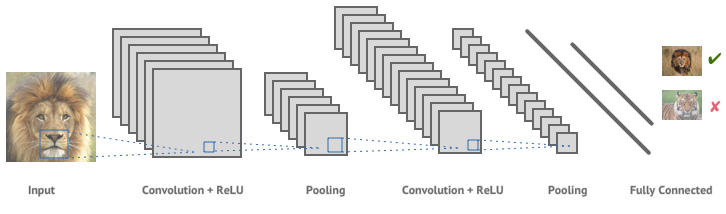
\includegraphics[width=1\textwidth]{img/convolutional_neural_network.png}
    \caption{Typische structuur van een Convolutional Neural Network \autocite{tejani}}
    \label{fig:structuur}
  \end{figure}

\subsection{Convolutional Layer}
\label{ssec:Convolutional Layer}
De eerst verborgen laag in een CNN is een convolutional layer. In deze laag wordt elk deel van de afbeelding vermenigvuldigd door bepaalde filters, een filter schuift of convoleert als het ware over de afbeelding. De bedoeling van een filter is om een feature of kenmerk te detecteren in een afbeelding. Dit kan gaan van eenvoudige herkenbare vormen zoals randen en bepaalde curves tot complexere structuren zoals ogen en oren. Het resultaat van de vermenigvuldiging geeft een quotering in hoeverre de feature aanwezig is. Nadat de filter over alle locaties van de invoer heeft geschoven vormen alle resultaten één nieuwe matrix. In de convulotional layer wordt één afbeelding omgezet naar een groep gefilterde afbeeldingen, afhankelijk van het aantal filters. Deze output wordt de input voor de volgende verborgen laag \autocite{becominghuman}.
Figuur \ref{fig:featuremap} toont een mooi voorbeeld van een feature map waarbij de filter randen detecteerde op een afbeelding van een tijger.
\begin{figure}[h!]
    \centering
        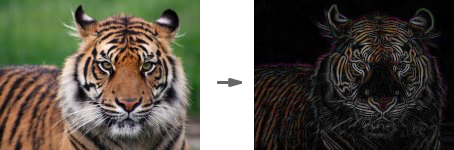
\includegraphics[width=0.5\textwidth]{img/tiger_edge_detection.png}
    \caption{Originele afbeelding gefilterd naar een feature map \autocite{tejani}}
    \label{fig:featuremap}
  \end{figure}

\subsection{Nonlinair Layer}
\label{ssec:Nonlinair Layer}
Deze laag ontvangt als input een verzameling van gefilterde afbeeldingen of ‘feature maps’. Aangezien de filter of functie uit de vorige laag linair is, kan het resultaat op een deel van de afbeelding ook negatief zijn. De nonlinair layer zet de linaire convolutielaag om naar een niet-linaire laag door een gelijkrichterfunctie, ReLu (Rectified Linear Unit) toe te passen. Deze functie zet alle negatieve waarden om naar de nulwaarde \autocite{cadence}.

\subsection{Pooling Layer}
\label{ssec:Pooling layer}
Pooling, of ook wel subsampling genoemd wordt gebruikt om de dimensie of grootte van de feature maps te verkleinen. In deze laag wordt het vaakst max-pooling toegepast. Een filter met een bepaalde dimensie overloopt de volledige feature map en haalt de maximum waarde daaruit. Net zoals in de nonlinair layer wordt de functie toegepast op elke feature map in de groep van feature maps die de convolutional layer als output gaf. Deze laag wordt gebruikt om de gebieden die het minst overeenstemmen met de filters uit de convolutionele laag te verwijderen om zo de berekeningen in het netwerk te verminderen \autocite{jeremy}.

\subsection{Fully Connected Layer}
\label{ssec:Fully Connected Layer}
De drie voorgaande verborgen lagen worden steeds na elkaar uitgevoerd. Aan het eind van het netwerk wordt de fully connected layer of softmax layer toegepast. Deze laag krijgt als input een groep op hoog niveau gefilterde afbeeldingen en bekijkt welke functies het meest overeenkomen met een bepaalde klasse. Het geeft een vector terug met de waarschijnlijkheid dat de afbeelding tot die klasse behoort, per klasse terug. Als het netwerk de grootste waarschijnlijkheid geeft dat een afbeelding een vogel is, dan zal de fully connected layer hoge waarden krijgen voor een feature die een snavel, een vleugel of iets dergelijk herkend \autocite{ujjwalkarn}.

\section{Transfer Learning}
\label{sec:Transfer Learning}

Om een CNN te ontwikkelen is een grote dataset gepaard met veel tijd nodig. Zelfs met sterke grafische kaarten kan het tot enkele weken duren alvorens het neurale netwerk getraind en voldoende nauwkeurig is. Transfer learning is een techniek die vaak gebruikt wordt om een CNN te ontwikkelen met een eigen kleinere dataset. Bovendien vraagt het toepassen van transfer learning aanzienlijk minder tijd \autocite{datacamp}.

De techniek hergebruikt een neuraal netwerk dat reeds getraind is met een enorme hoeveelheid data. Een veelvoorkomende dataset die wordt gebruikt om een neuraal netwerk te trainen is ImageNet, de set bevat meer dan één miljoen afbeeldingen onderverdeeld onder duizend categorieën. De bekenste modellen die met betreffende dataset getraind werden zijn VGG, ResNet en Inception, waar uit onderzoek wordt vastgesteld dat momenteel Inception v4 het meest nauwkeurige netwerk is \autocite{arxiv}.

Om een eigen classificatie model te ontwikkelen kan het voorgetrainde model gebruikt worden als 'fixed feature extractor' of om te 'finetunen'.

\subsection{Fixed feature extractor}
\label{ssec:Fixed feature extractor}

Wanneer het voorgetrainde netwerk gebruikt wordt als fixed feature extractor om een nieuw model te creëren, worden alle verborgen lagen behouden in het netwerk. Enkel de bovenste laag, de fully connected layer wordt verwijderd. Daarna wordt het netwerk gebruikt om met behulp van de nieuwe dataset een nieuwe output laag te trainen. Zo kan een netwerk dat auto’s herkent hergebruikt worden om vrachtwagens te herkennen. Deze benadering wordt vooral gebruikt wanneer de nieuwe dataset klein is \autocite{webcourse}.

\subsection{Fine-tuning}
\label{ssec:Fine-tuning}

Als fine-tuning wordt toegepast op een voorgetraind netwerk dan wordt niet alleen de fully connected layer vervangen, maar worden ook andere lagen aangepast om betere resultaten te bekomen. De eerste lagen die eenvoudige features detecteren zullen worden behouden. Diepere lagen die abstracte features waarnemen worden bijgeschaafd om specifieke features te achterhalen uit de nieuwe dataset. Op een model dat enkele hondenrassen herkend kan fine-tuning worden toegepast om veel meer hondenrassen te onderscheiden. Deze methode wordt meestal gebruikt wanneer er voldoende data beschikbaar is \autocite{cs231n}.


%%=============================================================================
%% Methodologie
%%=============================================================================

\chapter{Methodologie}
\label{ch:methodologie}

%% TODO: Hoe ben je te werk gegaan? Verdeel je onderzoek in grote fasen, en
%% licht in elke fase toe welke stappen je gevolgd hebt. Verantwoord waarom je
%% op deze manier te werk gegaan bent. Je moet kunnen aantonen dat je de best
%% mogelijke manier toegepast hebt om een antwoord te vinden op de
%% onderzoeksvraag.

\section{Opbouw van het onderzoek}
\label{sec:Opbouw van het onderzoek}

Dit onderzoek vergelijkt drie frameworks voor afbeeldingclassificatie. Er wordt onderzocht of eenvoudig implementeerbare frameworks even nauwkeurig resulteren als complexere frameworks. De drie frameworks worden getraind met negen producten uit de Feestwinkel, te Oudenaarde. De producten worden onderverdeeld in drie groepen: kleine producten, middelgrote producten en grote producten. Per groep wordt er voor elk framework een eigen classificatiemodel gecreëerd.

Als eerste framework is er gekozen voor een standaard machine learning bibliotheek. Onder deze noemer vallen frameworks zoals Caffe, Torch, Theano en Tensorflow. In dit onderzoek is gekozen voor Tensorflow, het scoort naast Theano het beste rekening houdend met snelheid, classificatie nauwkeurigheid en complexiteit van implementatie \autocite{researchgate}. Bovendien is er heel wat informatie te vinden op het web omtrent het toepassen van Tensorflow voor verschillende doeleinden \autocite{huyen}. De andere twee frameworks die worden toegepast in dit onderzoek zijn Turi Create en Microsoft Custom Vision. Deze frameworks zijn respectievelijk eenvoudiger in het ontwikkelen van een eigen afbeeldingclassificatie model. De drie frameworks zijn gratis te gebruiken. 

Nadat een eigen classificatie model getraind is met de trainingsdata per groep van producten, zal het model geëxporteerd worden naar een CoreML model. Het CoreML framework is gelanceerd door Apple op het \acrshort{WWDC} 2017. Het is een nieuwe toepassing in iOS 11 en het zorgt ervoor dat ontwikkelaars gemakkelijk machine learning models kunnen uitvoeren in hun applicaties. Zo ondersteund ook CoreML functies zoals gezichts- herkenning en tekstherkenning \autocite{coreml}. 

Vervolgens wordt per reeks van producten de drie bijhorende modellen getest op nauwkeurigheid en vergeleken met elkaar met behulp van een testapplicatie in iOS en testafbeeldingen. Hierdoor kan de eerste deelonderzoeksvraag beantwoord worden.

Na voltooiing van de vergelijking wordt een het best scorende en meest toepasbare framework gebruikt om enkele producten te trainen zodat een demoapplicatie om producten te herkennen ontwikkeld kan worden. De applicatie zal vervolgens uitgeprobeerd worden door klanten. Achteraf krijgen de consument enkele vragen met betrekking tot de applicatie zodat ook de laatste deelonderzoeksvragen een antwoord krijgen. 
\section{Frameworks}
\label{sec:Frameworks}

\subsection{Tensorflow}
\label{ssec:Tensorflow}

Tensorflow is open source deep learning framework door Google. Het is oorspronkelijk ontwikkeld in 2015 door het Google Brain Team om onderzoek te doen naar zowel machine learning, deep learning en neurale netwerken. In 2017 is de eerste open source versie van Tensorflow uitgebracht. Tensorflow wordt onder andere gebruikt voor tekstherkenning en stemherkenning maar ook voor afbeeldingclassificatie. De gemakkelijkste en de meest complete \acrshort{API} van dit framework is de Python \acrshort{API}, maar Tensorflow levert ook nog een API’s in Java, C++ en Go \autocite{introTensorflow}.

Om een aangepast model voor afbeeldingclassificatie te ontwikkelen past Tensorflow de transfer learning techniek toe met 'fixed feature extractor'. Het voorgetrainde model dat standaard benut wordt is Inception v3, die op basis van de dataset van ImageNet getraind werd. Tensorflow geeft echter wel de mogelijkheid om ook andere netwerken te hanteren zoals NASNet. In vergelijking met de andere twee frameworks heeft Tensorflow geen ingebouwde functie om het model te exporteren naar het CoreML-formaat \autocite{deeplearningTensor}.

\subsection{Turi Create}
\label{ssec:Turi Create}

Apple kocht in 2016 het bedrijf Turi over. Kort daarna gaf Apple het framework Turi Create vrij voor het publiek \autocite{9to5mac}. Apple beweert dat men met hun framework geen deskundige in machine learning hoeft te zijn. Een eigen afbeeldingclassificatie model kan gebouwd worden in enkele lijnen Python. Daarnaast kan het framework gebruikt worden voor onder andere objectdetectie en tekstclassificatie \autocite{githubturi}.

Turi Create functioneert volledig gelijklopend zoals Tensorflow. Het past ook transfer learning, met het verschil dat het dit framework gebruik maakt van het convolutional neural network ResNet-50 en niet Inception v3 \autocite{hackermoon}. Uit een vergelijkende studie van de nauwkeurigheid van verschillende \acrshort{CNN}’s scoort Inception v3 met een nauwkeurigheid van 79\%, waar ResNet-50 scoort met 76\% \autocite{arxiv}.

\subsection{Microsoft Custom Vision}
\label{ssec:Microsoft Custom Vision}

Microsoft lanceerde de Custom Vision API in 2017. De \acrshort{API} is een uitbreiding op de Microsoft Azure Cognitive Services, een verzameling van verschilllende machine learning \acrshort{API}’s. Ontwikkelaars kunnen op die manier eenvoudiger functies van artificiële intelligentie toepassen in hun applicaties. Zo kunnen de \acrshort{API}’s gebruikt worden voor onder andere gezichts-, en spraakherkenning. Maar ook video- en emotiedetectie. Daarnaast kunnen de services benut worden voor tekstanalyse en taalbegrip \autocite{cognitiveservices}.

De Custom Vision Service wordt gebruikt voor het eenvoudig trainen of verbeteren van eigen afbeeldingclassificaties. Deze service is in de vorm van een webapplicatie en vereist geen enkele kennis omtrent machine learning. Bovendien is er geen code nodig om een eigen model te ontwikkelen. Er dienen slechts enkele afbeeldingen per klasse online te worden geplaatst en de afbeeldingclassificatie wordt in luttele minuten getraind. Nadat het model getraind is kan het ook eenvoudig geëxporteerd worden naar het CoreML formaat of andere formaten \autocite{appliedies}.

De details over hoe Microsoft erin slaagt om met een ettelijk aantal afbeeldingen een nauwkeurig classificatiemodel te creëren houden ze voor zich. Al worden er in sommige blogpost geschreven dat Custom Vision ook de techniek transfer learning toepassen met behulp van het \acrshort{CNN} ResNet-50. Vooral omdat Microsoft Bing hetzelfde netwerk gebruikt voor afbeeldingherkenning \autocite{praeclarum}.









% Voeg hier je eigen hoofdstukken toe die de ``corpus'' van je bachelorproef
% vormen. De structuur en titels hangen af van je eigen onderzoek. Je kan bv.
% elke fase in je onderzoek in een apart hoofdstuk bespreken.

%\input{...}
%\input{...}
%...

%%=============================================================================
%% Conclusie
%%=============================================================================

\chapter{Conclusie}
\label{ch:conclusie}

%% TODO: Trek een duidelijke conclusie, in de vorm van een antwoord op de
%% onderzoeksvra(a)g(en). Wat was jouw bijdrage aan het onderzoeksdomein en
%% hoe biedt dit meerwaarde aan het vakgebied/doelgroep? Reflecteer kritisch
%% over het resultaat. Had je deze uitkomst verwacht? Zijn er zaken die nog
%% niet duidelijk zijn? Heeft het onderzoek geleid tot nieuwe vragen die
%% uitnodigen tot verder onderzoek?

%\lipsum[76-80]



%%=============================================================================
%% Bijlagen
%%=============================================================================

\appendix

%%---------- Onderzoeksvoorstel -----------------------------------------------

\chapter{Onderzoeksvoorstel}

Het onderwerp van deze bachelorproef is gebaseerd op een onderzoeksvoorstel dat vooraf werd beoordeeld door de promotor. Dat voorstel is opgenomen in deze bijlage.

% Verwijzing naar het bestand met de inhoud van het onderzoeksvoorstel

%%%---------- Inleiding ---------------------------------------------------------

\section{Introductie} % The \section*{} command stops section numbering
\label{sec:introductie}

Als u afgelopen jaar een online aankoop verricht hebt, dan bent u wellicht vertrouwd met de voordelen hiervan. U kon de huidige stock raadplegen, snel een ander kleur van het product kiezen, en mogelijks is uw aankoop zelfs gratis geleverd bij uw thuis. Daarnaast werden u waarschijnlijk bijpassende producten aanbevolen, of er werd getoond welke producten andere klanten kochten. Dit zijn beide toepassingen op de verkooptechniek Cross-selling. 
Deze techniek laat klanten ook effectief meer kopen, 35\% van de inkomsten van Amazon wordt bekomen door het aanbevelings-algoritme ~\autocite{Amazon}. \\~\\
Een fysieke winkel wordt op dergelijke algoritmen beperkt. Alleen verkopers kunnen andere producten aanbevelen wanneer ze een bezoeker helpen. Echter wordt niet elke klant bijgestaan door een verkoper. Dit onderzoek gaat na of een mobiele applicatie met product herkenning de fysieke winkel kan helpen om toch soortgelijke technieken toe te passen. Ik wil dit onderzoek zowel op commercieel als technisch vlak uitvoeren. Daarom bestaat het onderzoek uit volgende onderzoeksvragen:  
\begin{itemize}
  \item Wat is de nauwkeurigste Custom Image Classifier toepassing?
  \item Wordt productherkenning als hulpmiddel beschouwd?
  \item Beïnvloed productherkenning het koopgedrag van de consument?
\end{itemize}
\  \\
Samengevat zal er dus onderzocht worden of productherkenning een meerwaarde biedt aan een fysieke winkel en aan de consument. Op technisch vlak wordt er vooral aangetoond welk Machine Learning framework men best gebruikt bij implementatie. 

%---------- Stand van zaken ---------------------------------------------------

\section{State-of-the-art}
\label{sec:state-of-the-art}

Onderzoek en vergelijkingen van bestaande Machine Learning frameworks zijn uiteraard al uitgevoerd. Zo zijn “Tensorflow”, “Keras”, “Caffe”, “SciKit-Learn” en andere frameworks al verschillende keren met elkaar vergeleken ~\autocite{Deeplearning}.
Dit onderzoek zal maar een onderdeel van Machine Learning onderzoeken, namelijk “Image Classification”. Bij elk van opgesomde frameworks is die classificatie mogelijk. In 2017 kwam Apple met de release van “Turi Create”, een framework dat het eenvoudiger maakt om Machine Learning models te ontwikkelen zonder daarin een deskundige te zijn ~\autocite{9to5}. 
Ook met dit framework is classificatie mogelijk, maar het heeft nog steeds andere toepassingen ook. Hetzelfde jaar bracht Microsoft “Custom Vision” op de markt, een Machine Learning framework dat enkel en alleen het classificeren van afbeeldingen heeft als doelstelling ~\autocite{Microsoft}.
\\~\\
Dergelijk onderzoek naar de prestaties van “Turi Create” en “Custom Vision” is nog niet uitgevoerd. Aangezien dit onderzoek niet alleen de focus legt op de nauwkeurigheid van de frameworks, maar ook op de implementatie ervan zal een complex machine learning framework “Tensorflow” vergeleken worden met een eenvoudiger framework “Turi Create”. Daarnaast worden beide frameworks vergeleken met “Custom Vision” die alleen afbeelding classificatie heeft als toepassing. 
% Voor literatuurverwijzingen zijn er twee belangrijke commando's:
% \autocite{KEY} => (Auteur, jaartal) Gebruik dit als de naam van de auteur
%   geen onderdeel is van de zin.
% \textcite{KEY} => Auteur (jaartal)  Gebruik dit als de auteursnaam wel een
%   functie heeft in de zin (bv. ``Uit onderzoek door Doll & Hill (1954) bleek
%   ...'')


%---------- Methodologie ------------------------------------------------------
\section{Methodologie}
\label{sec:methodologie}

De eerste onderzoeksvraag gaat de nauwkeurigheid van de 3 frameworks na. Elk framework zal getraind worden op negen producten. Drie gelijkaardige kleine producten, drie gelijkaardige middelgrote producten en drie gelijkaardige grote producten. Daarna zal een demo applicatie gebruikt worden om een product van elke grootte 30 keer te scannen voor alle frameworks. De waarschijnlijkheid dat een framework het product herkend zal worden bijgehouden worden. Om antwoord te geven op de andere onderzoeksvragen zal een andere applicatie ontwikkeld worden. De applicatie zal gebruikmaken van het best scorende framework bij vorige onderzoeksvraag. Het framework zal voldoende getraind worden om een aantal producten zodat klanten van een fysieke winkel producten kunnen gaan scannen. De applicatie zal het product herkennen en hierbij info geven zoals het aantal stuks in voorraad en mogelijke bijproducten. Daarna zal zullen de gebruikers gevraagd worden of ze dit een hulpmiddel vinden en of ze de applicatie in de toekomst nog zullen gebruiken. Verder zal gevraagd worden of hun koopgedrag beïnvloed werd door het weergeven van mogelijke bijproducten/aanbevelingen.  

%---------- Verwachte resultaten ----------------------------------------------
\section{Verwachte resultaten}
\label{sec:verwachte_resultaten}

Bij de eerste onderzoeksvraag wordt er verwacht dat alle frameworks ongeveer even goed zullen scoren. Op commercieel vlak zal de applicatie vooral aanslaan bij jongere mensen die het gebruik van een smartphone gewoon zijn. Er wordt niet verwacht dat de mobiele applicatie even sterke invloed zal hebben op het koopgedrag van de consument dan een online webwinkel. 

%---------- Verwachte conclusies ----------------------------------------------
\section{Verwachte conclusies}
\label{sec:verwachte_conclusies}

Wanneer de verwachte resultaten kloppen, dan mag er geconcludeerd worden dat “Custom Vision” van Microsoft het beste framework is om productherkenning te implementeren in een fysieke winkel. Dit omdat het veel minder complex is om een machine te trainen op het herkennen van een specifiek product. Als deze toepassing aanslaat bij een grote groep klanten, dan zal productherkenning in de fysieke winkel zeker een toekomst hebben. Productherkenning kan worden uitgebreid tot de voedingssector, naast stockinformatie kunnen dan bijvoorbeeld ingrediënten en allergenen worden weergegeven. 

%%---------- Andere bijlagen --------------------------------------------------
% TODO: Voeg hier eventuele andere bijlagen toe
%\input{...}

%%---------- Referentielijst --------------------------------------------------

\printbibliography[heading=bibintoc]
%\addcontentsline{toc}{chapter}{\textcolor{maincolor}{\IfLanguageName{dutch}{Bibliografie}{Bibliography}}}

\end{document}
